\section{Data}

\subsection{Raw optical density data}
We start with the time series of the raw optical density (OD) measurements recorded during a single experimental run of a turbidostat. At consecutive (but not necessarily equidistant) time points, OD is recorded. This produces two vectors of real numbers:
\begin{itemize}
	\item the time points, $\{\text{tp}_n\;:\; n = 1,2, \ldots N_\text{total}\}$, and
	\item the OD values, $\{\text{od}_n\;:\; n = 1,2, \ldots N_\text{total}\}$.
\end{itemize}
Under normal operating conditions, the time series (tp, od) has the following features:
\begin{itemize}
	\item a long initial growth from a low OD value to the operating OD regime,
	\item sharp drops of OD, when it reaches a predefined threshold value,
	\item gradual growth of OD between sharps drops, and
	\item intermittent spikes of OD.
\end{itemize}

\subsection{Preprocessing}
Out of the four features of the raw (tp, od) time series, we wish to model only the gradual growth (and maybe the initial growth) phases. For this we filter the time series and partition it into non-overlapping regions by 
\begin{enumerate}
	\item Using heuristic filters to identify sudden changes of od, and remove the associated data points.
	\item Group uninterrupted series of data points into non-overlapping regions.
	\item Take the logarithm of OD.
\end{enumerate}
This produces the cleaned time series $(t, x)$ of $N$ data points:
\ba
	t &=& (t_1, t_2, \ldots t_N), \quad \text{where}\; t_n \in \mathds{R},\quad \text{and}\; t_n < t_{n+1}, \\
	x &=& (x_1, x_2, \ldots x_N), \quad \text{where}\; x_n = \log(\text{od}) \in \mathds{R},
\ea
and a list of $R$ regions, i.e. non-overlapping sets $\mathcal{R}_r$,
\be
	r \in \{1, 2, \ldots R\},\qquad \text{where each }\mathcal{R}_r = \{s(r), s(r) + 1, \ldots e(r) - 1, e(r)\} \subset \{1, 2,\ldots N\}
\ee
is a list of consecutive indexes, where $s(r)$ is the first and $e(r)$ is the last. The bottom panel of \reffig{fig:data} illustrates how a typical $(x,t)$ time series look like.

\newpage
\begin{figure}[h]
\centering
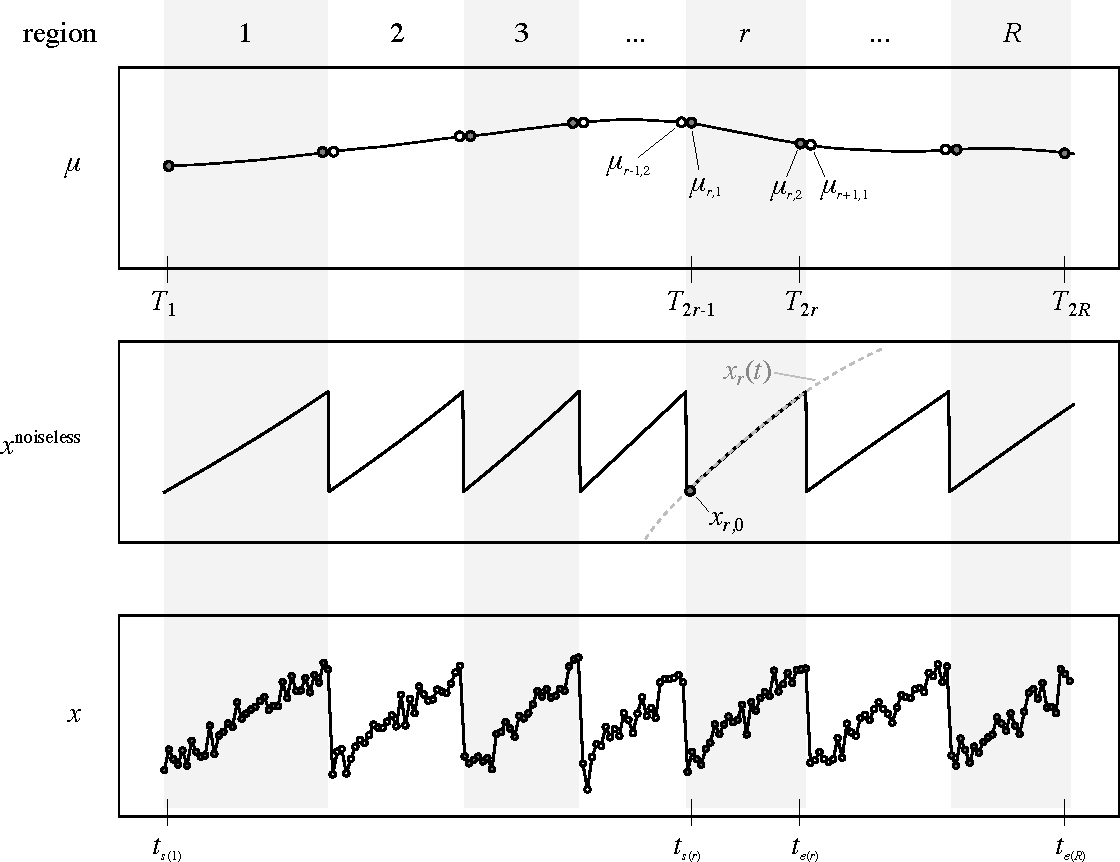
\includegraphics[width=\textwidth]{figs/data.pdf}
\caption{
	\label{fig:data}
	Illustration of the data expected by the model, which is described in the next section. {\bf (Top panel)} The growth rate $\mu$ changes gradually with time. {\bf (Middle panel)} The hidden $x^\text{noiseless}$ log-OD follows a saw-tooth-like behavior, where regions of gradual growth (between times $t_{s(r)}$ and $t_{e(r)}$ for each region $r$) are interrupted by sudden drops. {\bf (Bottom panel)}Due to measurement noise, the recorded $x$ log-OD values are distributed around the noiseless log-OD curve, where deviations are uncorrelated.
}
\end{figure}
\newpage
